% !TEX root = ps2_text.tex

\documentclass[12pt]{article}

% Geometry
\usepackage[a4paper, left=3cm, right=2.5cm, top=2.5cm, bottom=3cm]{geometry}

% Font encoding
\usepackage[utf8]{inputenc} % UTF-8 encoding
\usepackage[T1]{fontenc} % Font encoding
\usepackage{times}

% Math packages
\usepackage{amsmath} % Basic math symbols and environments
\usepackage{amssymb} % Additional math symbols
\usepackage{amsfonts} % Math fonts

% Text packages
\usepackage{parskip}
\setlength{\parskip}{1em}
\usepackage{hyperref}
\hypersetup{
    colorlinks=true,
    linkcolor=blue,
}

% Pictures
\usepackage{graphicx}
\usepackage{float}

% Lists
\usepackage{enumitem}
\setlist[itemize]{itemsep = -0.5em, topsep = -0.5em}

% Bibliography
%\usepackage{cite}

% Loops:
\usepackage{pgffor}

% Title and author
\title{Econometrics II - Problem Set 1}
\author{Ricardo Semião e Castro}
\date{05/2024}


\begin{document}

\maketitle

\section*{Question 1}

\subsection*{Item 1.}

\subsection*{Item 2.}

\subsection*{Item 3.}

\section*{Question 2}

\subsection*{Item 1.}

\subsection*{Item 2.}

\subsection*{Item 3.}

\section*{Question 3}

\subsection*{Item 1.}

\subsection*{Item 2.}

\subsection*{Item 3.}

\section*{Question 4}

First of all, we can plot the historic values and the auto-correlation of the series, to see that it has a clear positive tendency, and a lot of memory. These are signs that indicate a possible unit root.

\begin{figure}[H]
    \centering
    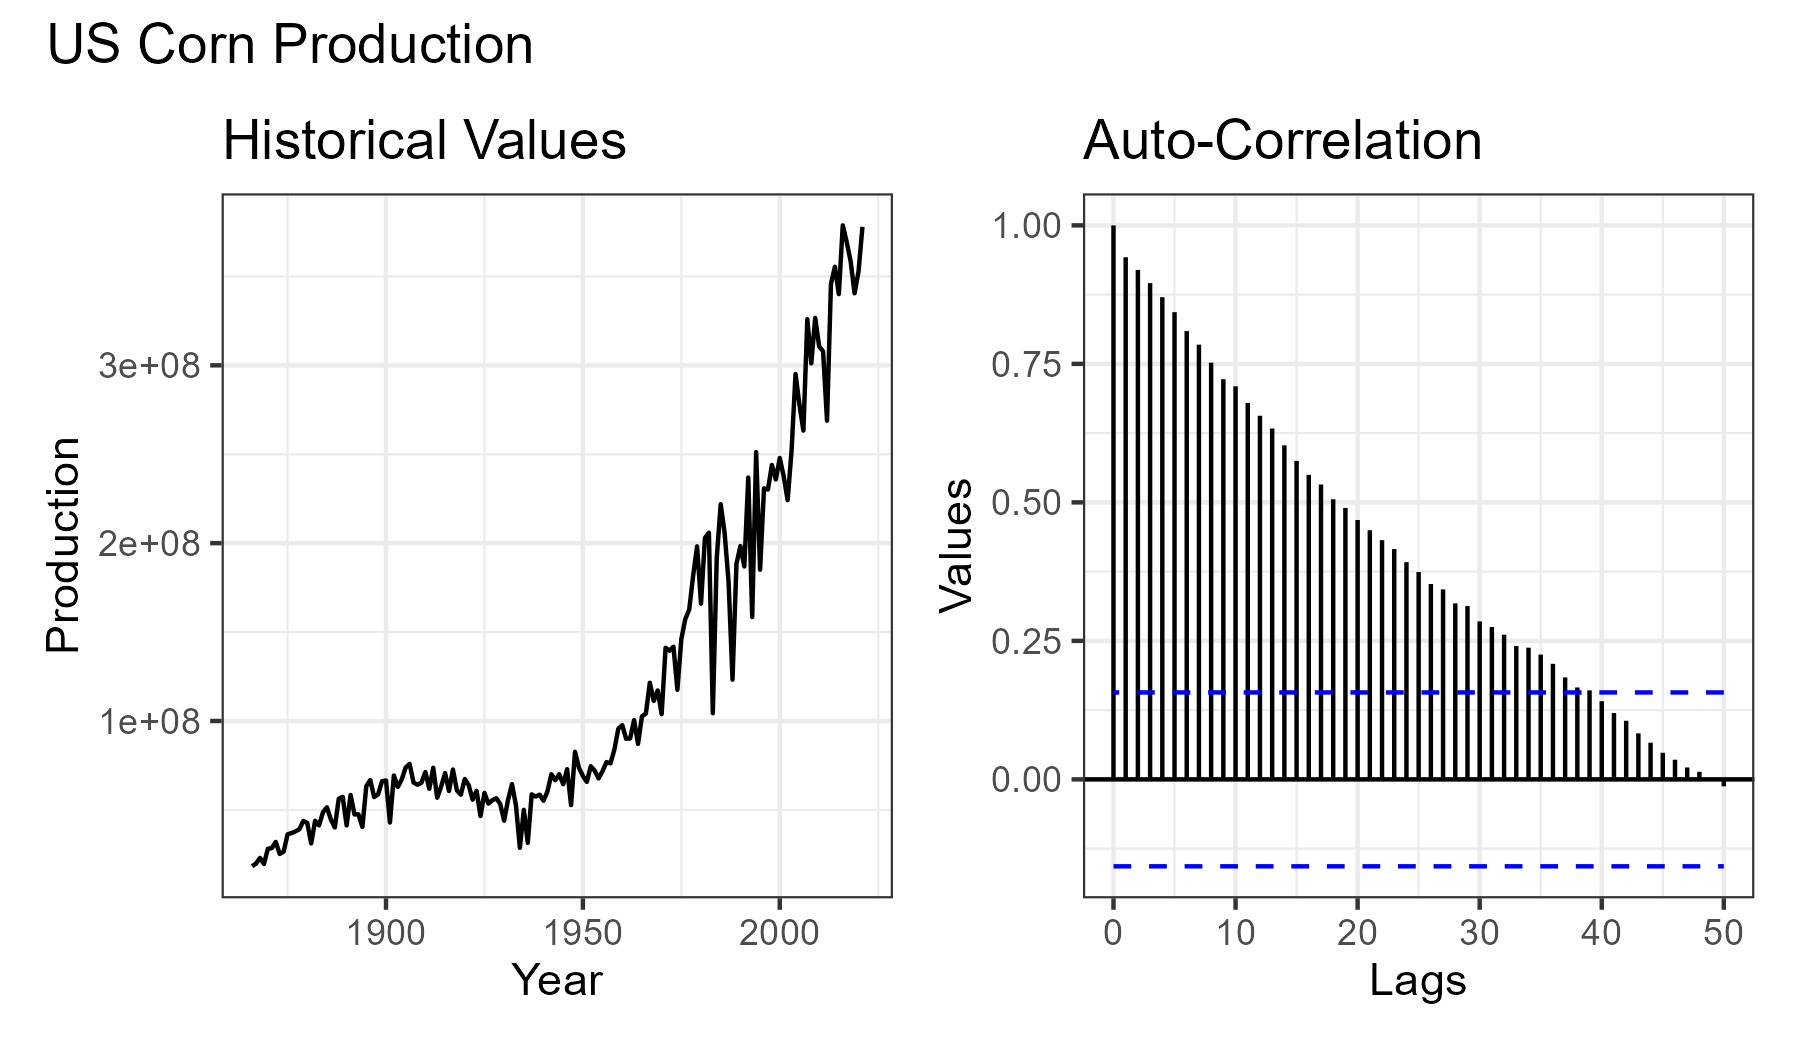
\includegraphics[width=0.8\textwidth]{figures/corn_prod.png}
\end{figure}

Now for the test, we use the function \href{https://rdrr.io/cran/aTSA/man/adf.test.html}{aTSA::adf.test}, that tests three specifications:

\begin{itemize}
    \item Type 1: A linear model with no drift nor linear trend.
    \item Type 2: A linear model with drift but no linear trend.
    \item Type 3: A linear model with drift and linear trend.
\end{itemize}

Each of them with a multitude of lags of the first difference of the serie. In our case, I set the maximum number of lags to 4, given the yearly nature of the data.

Test statistic is the estimated coefficient of the lagged time serie, divided by its standard error. The null hypothesis is that the coefficient is equal to zero, which would indicate an $I(0)$ process.

The results are presented below, with p-values in parenthesis. We can see that the null hypothesis is rejected for all three specifications, for any number of lags, which indicates that the series has a unit root.


% Table created by stargazer v.5.2.3 by Marek Hlavac, Social Policy Institute. E-mail: marek.hlavac at gmail.com
% Date and time: sáb, mai 18, 2024 - 17:42:28
\begin{table}[!htbp] \centering 
  \caption{} 
  \label{} 
\begin{tabular}{@{\extracolsep{5pt}} cccc} 
\\[-1.8ex]\hline 
\hline \\[-1.8ex] 
Lag & Type 1 & Type 2 & Type 3 \\ 
\hline \\[-1.8ex] 
0 & 0.61
(0.82) & -0.54
(0.86) & -2.74
(0.27) \\ 
1 & 2.08
(0.99) & 0.78
(0.99) & -1.16
(0.91) \\ 
2 & 3.01
(0.99) & 1.51
(0.99) & -0.53
(0.98) \\ 
3 & 3.91
(0.99) & 2.21
(0.99) & 0
(0.99) \\ 
4 & 4.87
(0.99) & 3.05
(0.99) & 0.54
(0.99) \\ 
\hline \\[-1.8ex] 
\end{tabular} 
\end{table} 


\end{document}
